\documentclass[../main.tex]{subfiles}

\begin{document}

\subsubsection*{Methodology}
    In this section we use a variable input power to the active medium of the HeNe Laser to analyse influence on the output power. We use a stepsize of $\delta I = 0.1\;\si{\mA}$ and a linear displacement in $15$ steps following $s(n) = -\delta I\cdot n + I_0$ with $I_0 = 6.5\;\si{\mA}$ being the initial current. Unfortunately we do not know the uncertainty of the current as it was not given in the manual. 
\subsubsection*{Data analysis}

    To convert from the initially measured current to the effectively used power we used the voltage $U_{\textit{in}} = (2.0\pm 0.1)\;\si{\kV}$ and the conversion formula $P_{\textit{in}}(I) = I \cdot U_{\textit{in}} + P_{fl}$. Unfortunately we did not measure the $P_{fl}$ offset coming from the flourescent light of the HeNe laser, which is why we have an extra uncertainty that we only involve qualitatively later on. 
    Because the used measurement tool to capture the current does not provide an uncertainty, we only used the given voltage error for the plots $x$ axis. In the $y$ axis we noted a compareably small error of $\SI{0.1}{\mW}$ during the experiment, which cannot be displayed against the data points. We assume it therefore to be negligible. Figure \ref{fig:output_power_over_input_power} shows the output power of the HeNe laser as a function of the input power.
    \begin{figure}[H]
        \centering
        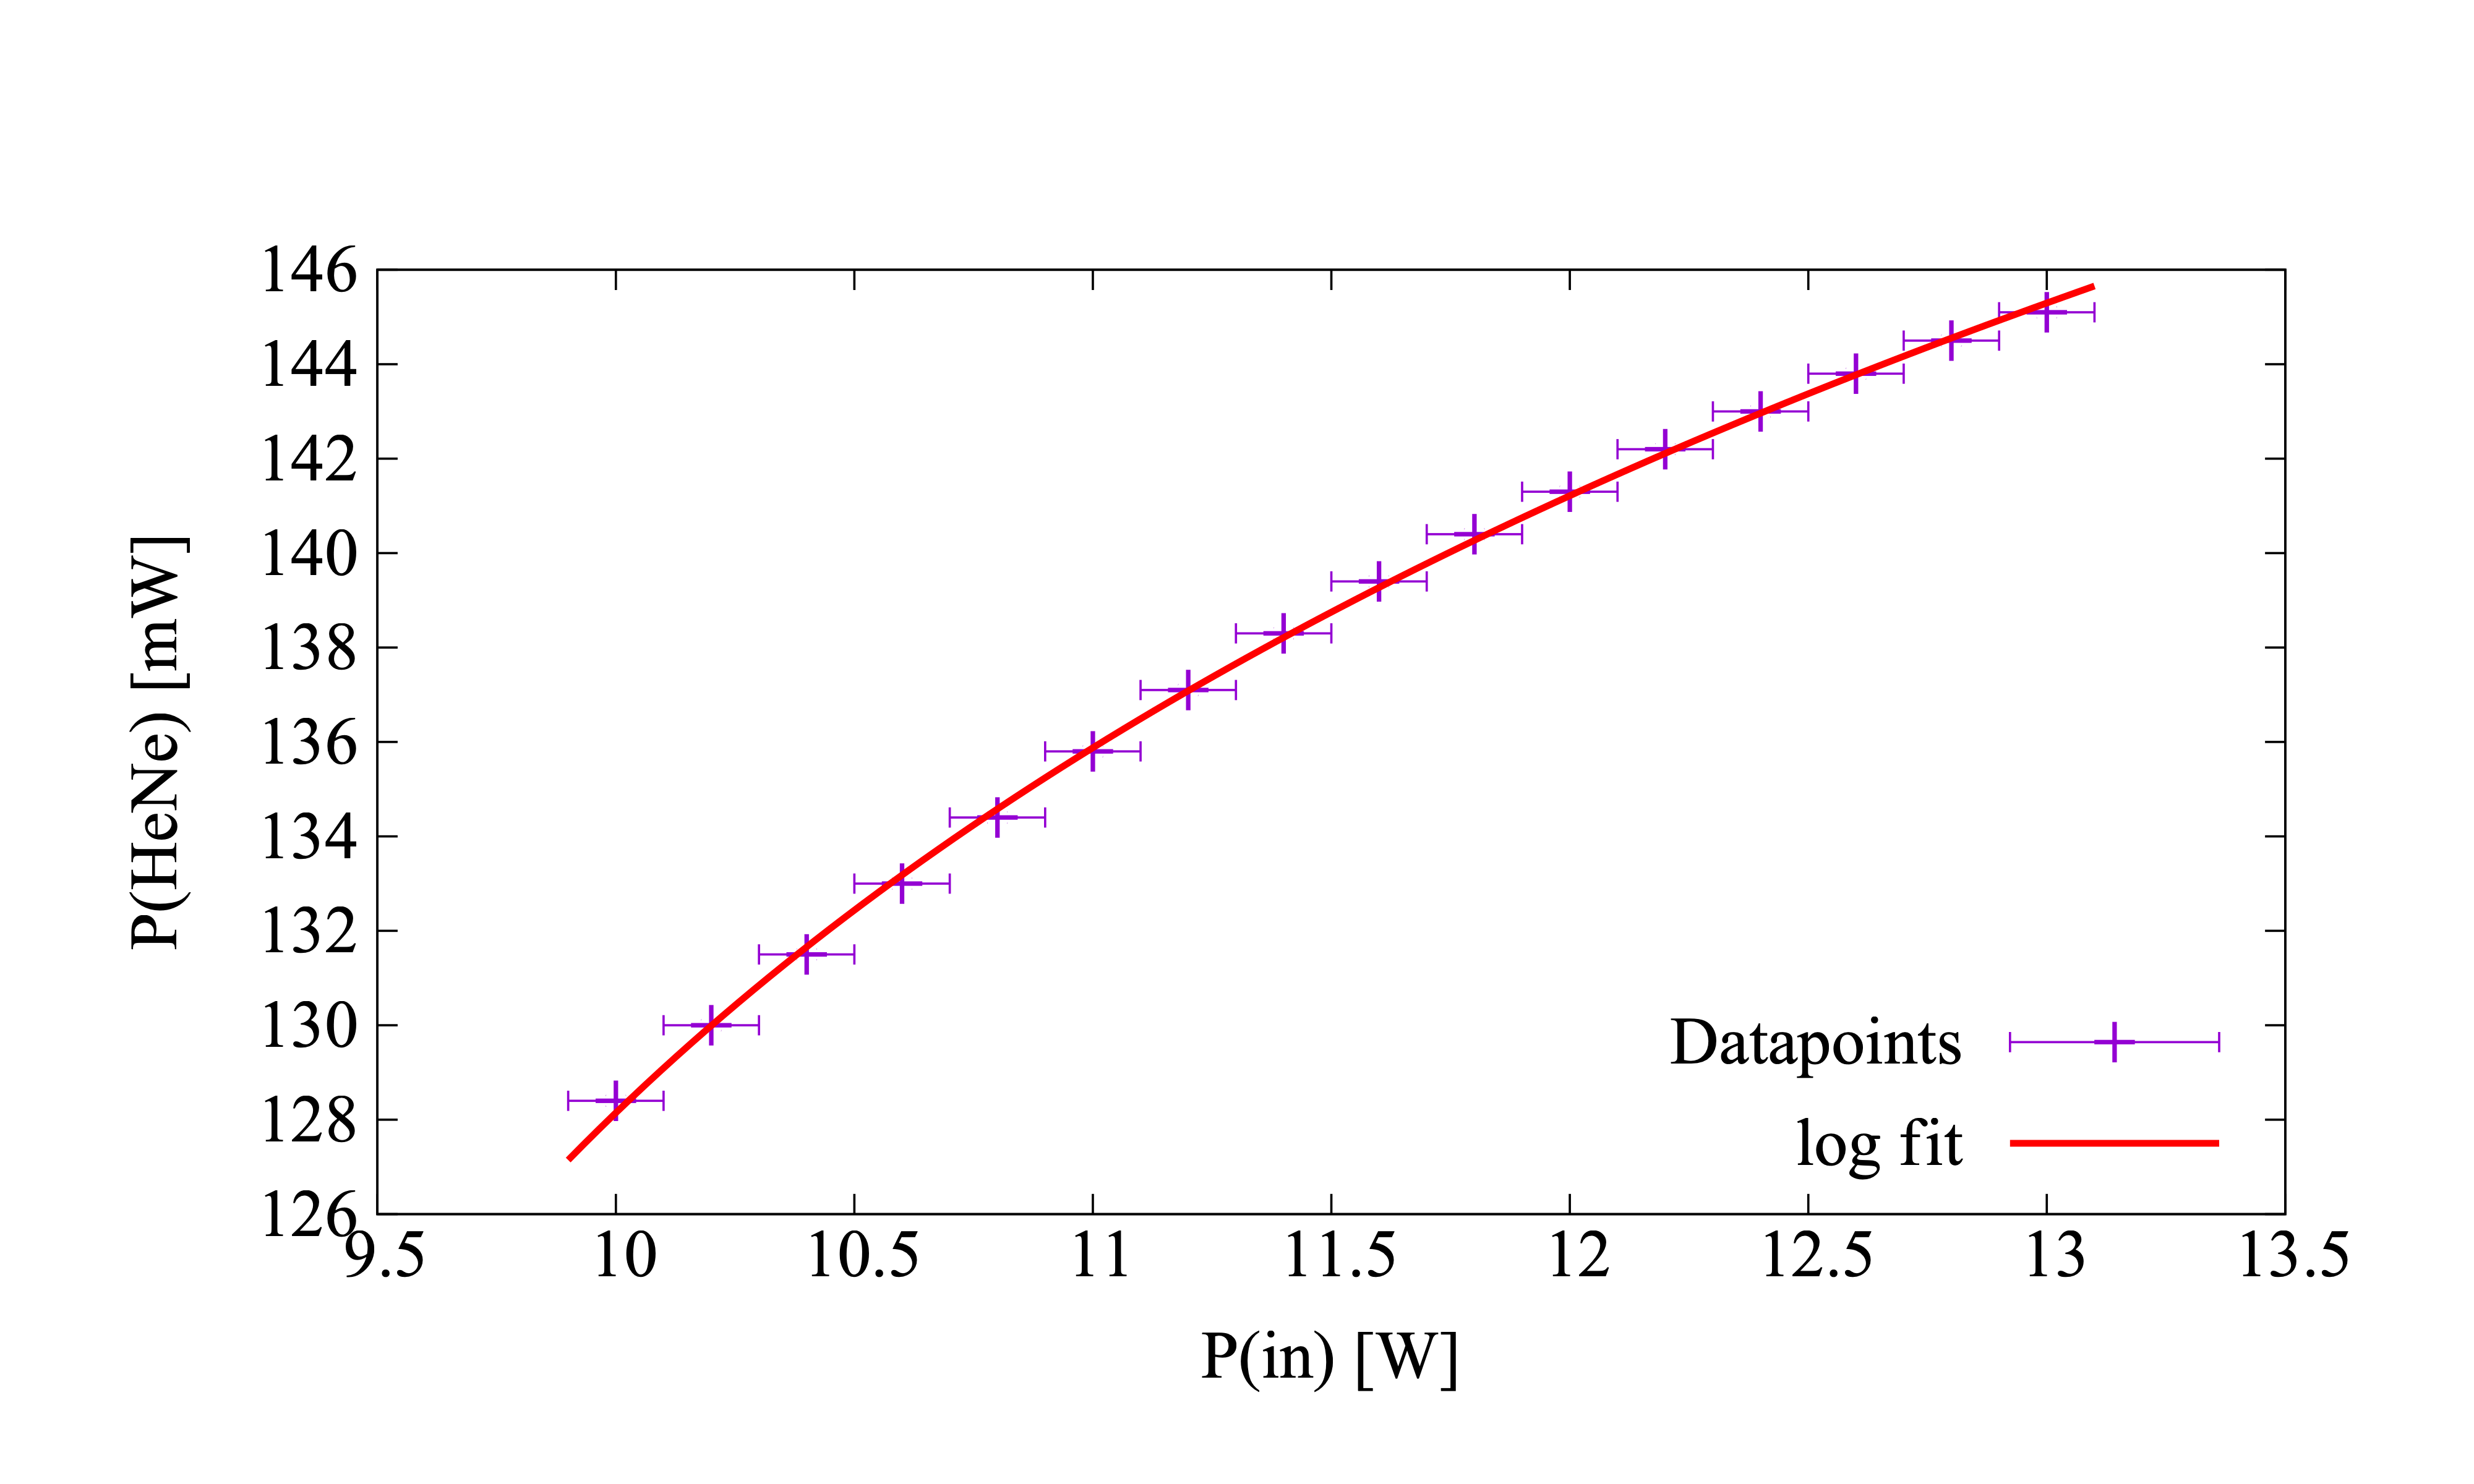
\includegraphics[width=0.8\textwidth]{Bilddateien/2/P(HeNe)overP(in)-log.png}
        \caption{The output power of the HeNe laser as a function of the input power.}
        \label{fig:output_power_over_input_power}
    \end{figure}
    Because the correct functional relationship between the input and output power is unknown, we used several fitting functions such as sqrt, ln and linear. The best approximation was achieved using ln, so let $f_a(x) := a_1\cdot \ln(a_2\cdot x + a_3) + a_4$ and $a$ be the fitting vector. Then table \ref{tab:fitting_vector_logfit} shows the fitting vector $a$ for the given rescaled dataset. 
    \begin{table}[H]
        \centering
        \begin{tabular}{|c|c|c|c}
            \hline
             & $a_i$ & $u(a_i)$ \\
            \hline\hline
            $a_1$ & $8.60188$ & $9.095$ \\
            $a_2$ & $2.88749$ & $6.693$ \\
            $a_3$ & $-27.5754$ & $62.23$ \\
            $a_4$ & $118.268$ & $5.013$ \\
            \hline
        \end{tabular}
        \caption{The fitting vector $a$ for the function $f_a$. We neglect the units as they are not relevant for the calculation.}
        \label{tab:fitting_vector_logfit}
    \end{table}
    To calulate the minimal input power $P_0$ required to achieve lasing we solve $0 = f_a(P_0)$. For this we use $f_a^{-1}=\fdef{(\exp((y-a_4)/a_1)-a_3)/a_2}{y\in\R}$ and uts uncertainty function as the sum of the squared partial derivatives of $f_a^{-1}$ times the squared uncertainty of the direction, i.a. $u(f_a^{-1}):=\fdef{\bbra{\sum_{i\in[4]}\partial_if_a^{-1}(y)^2\cdot u(a_i)^2}^{1/2}}{y\in\R}$. This yields us the result presented in table \ref{tab:minimal_input_power}. 
    \begin{table}[H]
        \centering
        \begin{tabular}{|c|cc|}
            \hline
            & $P_0$ & $u(P_0)$ \\
            \hline\hline
            Result & \SI{8.2087}{\W} & \SI{30.8496}{\W} \\
            \hline
        \end{tabular}
        \caption{The minimal input power $P_0$ required to achieve lasing.}
        \label{tab:minimal_input_power}
    \end{table}
    As we can clearly see the uncertainty of the calculation is much greater than itself, which indicates a suboptimal choice of the rastering range as it does not clearly extrapolate to the origin. The laser efficiency can be displayed as a function of the input current a.i. $q(I) := P_{\textit{out}}(I)/P_{\textit{in}}(I)$. With the uncertainty formular simularely defined as in $u(f_a^{-1})$ we get the plot shown in figure \ref{fig:efficiency_over_input_current}. 
    \begin{figure}[H]
        \centering
        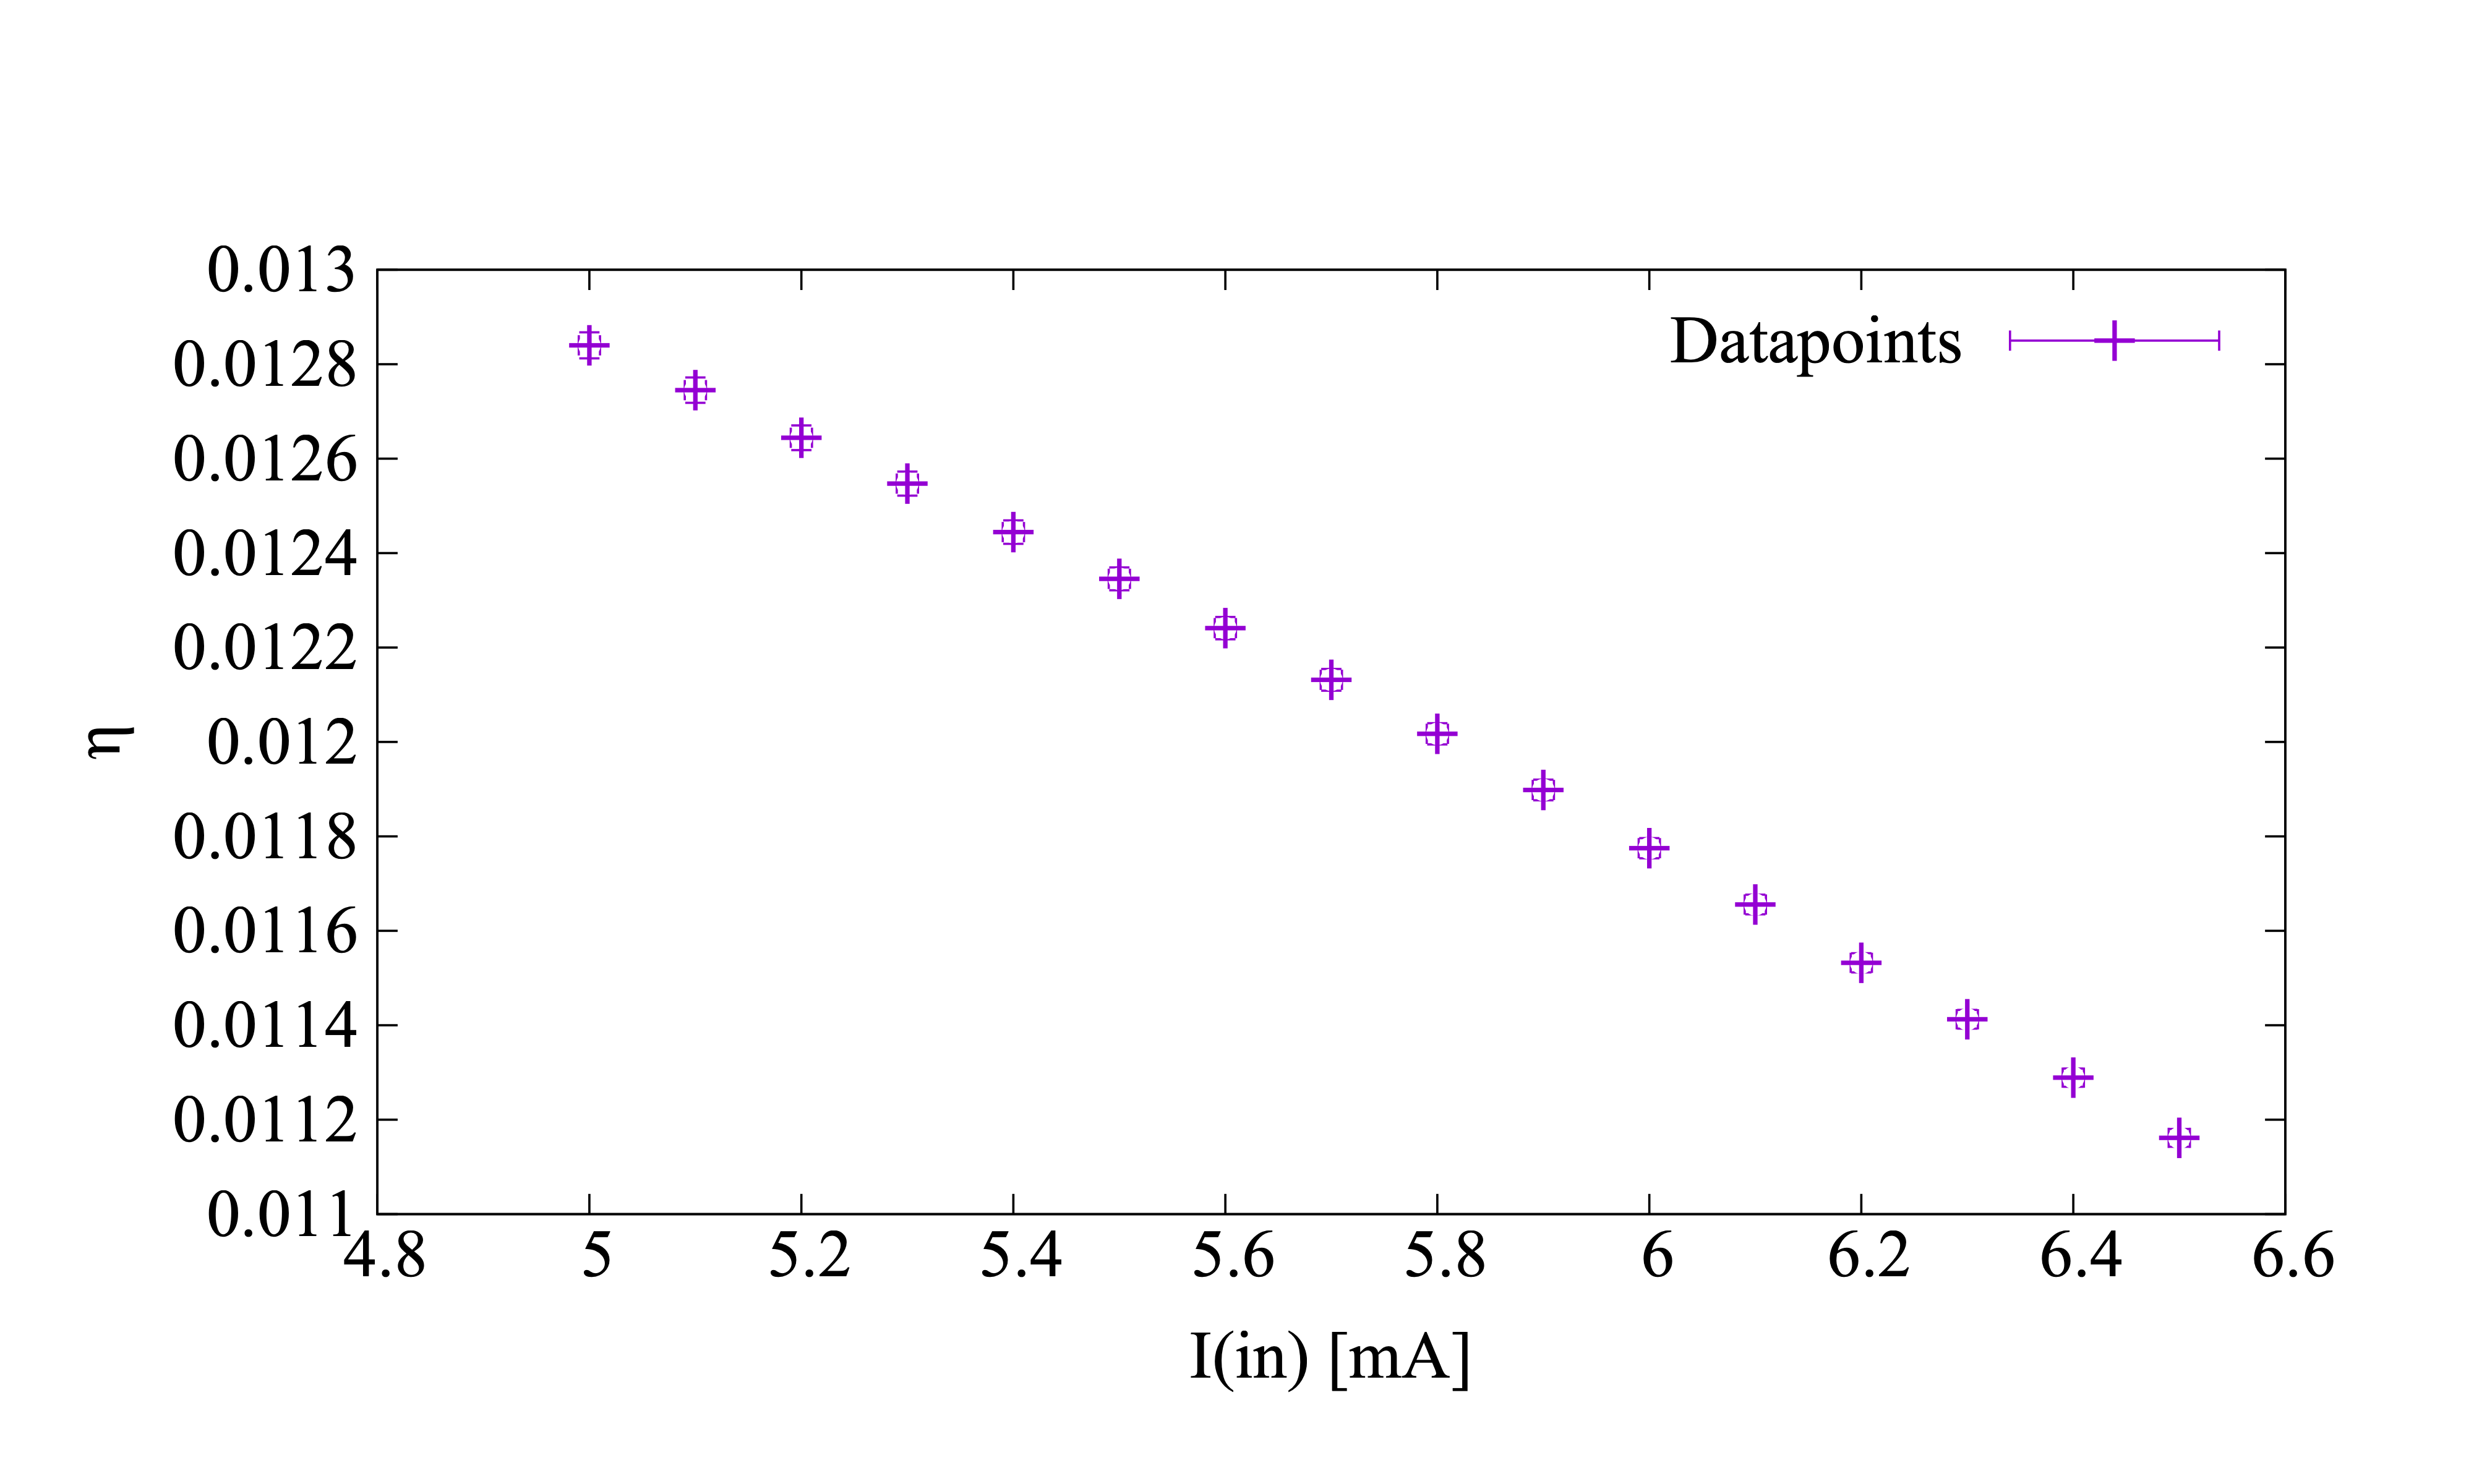
\includegraphics[width=0.8\textwidth]{Bilddateien/2/efficiency-over-in-current.png}
        \caption{The efficiency of the HeNe laser as a function of the input current.}
        \label{fig:efficiency_over_input_current}
    \end{figure}
    We can clearly observe its decline when using higher input currents and its generally low amplitude. 



\end{document}